\documentclass{article}
\usepackage[utf8]{inputenc}
\usepackage{polski}
\selecthyphenation{polish}
\usepackage{graphicx}
\usepackage[justification=raggedright, format=plain]{caption}
\usepackage{hyperref}
\usepackage{enumerate}
\usepackage{subfigure}
\graphicspath{ {./images/} }
\def\code#1{\texttt{#1}}

\title{Kodowanie słownikowe danych o strukturze bajtowej}
\author{Hubert Adamkiewicz}
\date{Styczeń 2021}

\begin{document}
\maketitle

\section{Opis problemu}
\label{sec:opis_problemu}
Zadanie polega na zrealizowaniu prostego kodera i dekodera wykorzystującego metodę LZ77
(dla ustalenia uwagi proszę stosować metodę w wariancie przedstawionym w materiałach
wykładowych).
Przyjmujemy następujące założenia:
\begin{enumerate}
\item Kodowane pliki mają strukturę bajtową (tzn. mogą zawierać dane z dowolnego
problemu, w którym występuje co najwyżej \textbf{256} różnych „komunikatów”).
\item Długość \textit{bufora słownika} wynosi \textbf{256} bajtów, a \textit{bufora wejściowego (look-ahead buffer)}
\textbf{15} bajtów, tzn. pojedynczy \textit{wskaźnik do słownika} ma rozmiar \textbf{2.5} bajta (\textbf{1} bajt
reprezentujący położenie kopii fragmentu znalezionej w słowniku czyli \textit{offset}, \textbf{0.5} bajta
do zakodowania \textit{długości kopii} oraz \textbf{1} bajt zawierający „komunikat” bezpośrednio po
znalezionym fragmencie).
\item Rozwiązanie ma mieć postać DWÓCH gotowych do użycia \\ funkcji/skryptów/aplikacji,
tzn. \textit{kodera} i \textit{dekodera}.
\item Koder ma dwa argumenty wejściowe, tzn. (1) nazwa wraz z rozszerzeniem
kodowanego pliku oraz (2) nazwa (wraz z dowolnie zdefiniowanym rozszerzeniem, na
przykład \textbf{.xxx}) pliku zakodowanego, który ma być zapisany w tym samym folderze,
co plik kodowany.
\item \textit{Dekoder} ma również dwa argumenty wejściowe, tzn. (1) nazwa (wraz z zastosowanym
rozszerzeniem, na przykład \textbf{.xxx}) dekodowanego pliku oraz (2) nazwa (wraz z
zadanym rozszerzeniem) pliku rozkodowanego, który ma być zapisany w tym samym
folderze, co plik dekodowany.
Zrealizowane rozwiązania powinny być przetestowane na wybranych przykładach (np. plikach
w formacie \textbf{.txt}).
\end{enumerate}

\section{Szczegóły implementacji}
\subsection{Koder}
Funkcjonalność kodera została zaimplementowana w pliku \textit{lz77\_encoder.py}. Aby uruchomić program należy mieć zainstalowany w systemie interpreter języka Python w wersji przynajmniej 2.7 oraz użyć polecenia \code{python lz77\_encoder.py plik\_wejsciowy plik\_wyjsciowy}. Jeżeli ścieżka do pliku wyjściowego nie będzie zawierała rozszerzenia, skrypt automatycznie przypisze rozszerzenie \textbf{.lz77}. Ponadto do polecenia można dodać parametr \code{-v} lub \code{--verbose}, który wyświetli w konsoli poszczególne kroki algorytmu LZ77 w formacie \textbf{$\langle$offset, length, next\_char$\rangle$} , gdzie:
\begin{itemize}
    \item \textit{offset} to pozycja najdłuższego znalezionego podciągu bufora look-ahead w buforze słownika (licząc od końca bufora słownika, czyli znaku najbliżej początku bufora look-ahead),
    \item \textit{length} to długość znalezionego najdłuższego podciągu znaków, które należy przepisać z bufora słownika,
    \item \textit{next\_char} to kolejny znak do zakodowania po przepisaniu wcześniej zdefiniowanego podciągu znaków.
\end{itemize}
Koder po zakończeniu swojej pracy wyświetla także informacje dotyczące stopnia uzyskanej kompresji, procent kompresji oraz średnią bitową. Wartości te zostaną przytoczone w sekcji analizy wyników działania kodera.
\\ Pewną niedogodnością korzystania z języka Python jest fakt, iż operuje on na bajtach, a nie bitach. Z tego powodu dane zapisywane są do plikach po 2 informacje jednocześnie, tak aby uzyskać całkowitą liczbę bitów do zapisu w zakodowanym pliku (w sekcji \ref{sec:opis_problemu} zaznaczono, że pojedyncza informacja powinna mieć długość \textbf{2.5 bajta}). 

\subsection{Dekoder}
Dekoder został zaimplementowany w pliku textit{lz77\_decoder.py}. Działa on analogicznie do kodera, zatem uruchamiany jest poleceniem \code{python lz77\_decoder.py plik\_zakodowany plik\_wyjsciowy} i tak samo jak koder posiada także opcjonalny parametr \code{--verbose} wyświetlający odczytane kroki algorytmu LZ77.
\\Dekoder zapisuje w pamięci zawartość pliku zakodowanego, a następnie pobiera z niego każdorazowo \textbf{2.5 bajta} danych, które dekoduje do jednego kroku algorytmu LZ77 i rozkodowany ciąg znaków dopisuje do tablicy danych wyjściowych. Na końcu pracy dekodera dane wyjściowe zapisane są do pliku o wskazanej w poleceniu ścieżce, co owocuje odtworzeniem pierwotnego pliku użytego jako wejście do kodera.

\subsection{Zapisane przykłady działania skryptów}
W katalogu z projektem znajdują się 3 podkatalogi zawierające zapisane przykłady użycia kodera i dekodera:
\begin{itemize}
    \item \textit{input} -- zawiera pliki wejściowe dla kodera LZ77,
    \item \textit{encoded} -- zawiera pliki z katalogu \textit{input} skompresowane przy użyciu kodera
    \item \textit{decoded} -- zawiera pliki z katalogu \textit{encoded} zdekodowane za pomocą dekodera
\end{itemize}
Są to pliki opisane w kolejnym rozdziale, które posłużyły do przetestowania poprawności oraz skuteczności zaimplementowanych narzędzi.

\section{Wyniki i wnioski}
Testy działania kodera i dekodera zostały przeprowadzone głównie na plikach wykorzystywanych podczas wykładów. Jako że na zajęciach skupialiśmy się głównie na obrazach i dźwiękach, do bazy plików wejściowych dołączone zostały również pliki tekstowe: "Lorem ipsum" (5 pierwszych akapitów), tekst powieści Adama Mickiewicza pt. "Pan Tadeusz, czyli ostatni zajazd na Litwie" oraz tekst dotyczący pojęcia \textit{strony obliczeniowej} w tłumaczeniu tekstów (źródło: \url{http://tlumaczeniamickiewicz.pl/o_stronie_obliczeniowej_2.pdf}).

\subsection{Kompresja plików tekstowych}
\begin{enumerate}
\item \textbf{Tekst powieści "Pan Tadeusz"} - wyniki kompresji:
    \begin{itemize}
        \item CR (stopień kompresji) = 1.16203778
        \item CP (procent kompresji) = 13.94\%
        \item BR (średnia bitowa) = 6.8845
    \end{itemize}
\item \textbf{"Lorem ipsum"} - wyniki kompresji:
    \begin{itemize}
        \item CR = 1.29839572
        \item CP = 22.98\%
        \item BR = 6.1614
    \end{itemize}
\item \textbf{"O stronie obliczeniowej"} - wyniki kompresji:
    \begin{itemize}
        \item CR = 1.28762770
        \item CP = 22.34\%
        \item BR = 6.2130
    \end{itemize}
\end{enumerate}

Kompresja tekstów przynosi zatem zysk w postaci około 20\%-owego zmniejszenia rozmiaru zakodowanego pliku, co na przykład w przypadku tekstu "Pana Tadeusza" pozwoliło na oszczędność w postaci \textbf{65.68kB} powierzchni dyskowej lub transferu danych.

\subsection{Kompresja obrazów (bitmap 8-bitowych)}
\begin{enumerate}
\item 
    \begin{figure}
       \minipage{0.30\textwidth}
            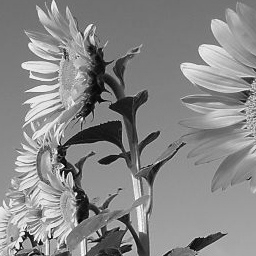
\includegraphics[width=\linewidth]{sunflow}
            \caption{SUNFLOW.bmp}
        \endminipage\hfill
        \minipage{0.30\textwidth}
            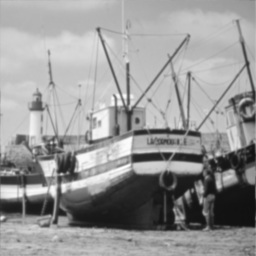
\includegraphics[width=\linewidth]{boats}
            \caption{BOATS.bmp}
        \endminipage\hfill
            \minipage{0.30\textwidth}
            
\includegraphics[width=\linewidth]{img1}
            \caption{img1.bmp}\hfill
        \endminipage
    \end{figure}
    \textbf{SUNFLOW.bmp} - wyniki kompresji:
    \begin{itemize}
        \item CR = 0.86708754
        \item CP = -15.33\%
        \item BR = 9.2263

    \end{itemize}
\item 
    \textbf{BOATS.bmp} - wyniki kompresji:
    \begin{itemize}
        \item CR = 0.94227315
        \item CP = -6.13\%
        \item BR = 8.4901

    \end{itemize}
\item
    \textbf{img1.bmp} - wyniki kompresji:
    \begin{itemize}
        \item CR = 5.44677024
        \item CP = 81.64\%
        \item BR = 1.4688
    \end{itemize}
\end{enumerate}
Analiza wyników kompresji obrazów algorytmem LZ77 wykazuje, że zakodowane pliki graficzne zazwyczaj mają większy rozmiar niż pliki wejściowe. Prawdopodobnie jest to spowodowane tym, że analizując obraz piksel po pikselu rzadko powtarza się dłuższa sekwencja takich samych wartości następujących po sobie bądź parametry kodera (długość bufora słownika i bufora wejściowego) są nieefektywne do kodowania tego typu informacji.
\\Warto natomiast zauważyć, że w sytuacji, gdy obraz zawiera powtarzalne wartości (tak jak w pliku \textit{img1.bmp}), to algorytm bardzo efektywnie je zapisuje zmniejszając rozmiar pliku zakodowanego ponad pięciokrotnie. Niestety, w praktyce takie bitmapy pojawiają się niezwykle rzadko, choć algorytm ten może znaleźć zastosowanie w kodowaniu obrazów zawierających kody kreskowe bądź kody QR.
\subsection{Kompresja sygnału audio (32-bit float, mono, 44100Hz)}
Co prawda implementacja została przygotowana do pracy z plikami zawierających 8-bitowe informacje o wartościach całkowitych, jednak działa ona bezpośrednio na danych w postaci binarnej. Postanowiłem zatem sprawdzić zachowanie zaimplementowanego kodera LZ77 w pracy z plikami przeznaczonymi dla poprzedniego projektu.
\begin{enumerate}
\item \textbf{icing.wav} - wyniki kompresji:
    \begin{itemize}
        \item CR = 0.76259250
        \item CP = -31.13\%
        \item BR = 10.4905

    \end{itemize}
\item \textbf{"music2.wav"} - wyniki kompresji:
    \begin{itemize}
        \item CR = 0.73465301
        \item CP = -36.12\%
        \item BR = 10.8895
    \end{itemize}
\item \textbf{"song.wav"} - wyniki kompresji:
    \begin{itemize}
        \item CR = 0.76278970
        \item CP = -31.10\%
        \item BR = 10.4878
    \end{itemize}
\end{enumerate}
Wyniki kompresji są tragiczne - zakodowane pliki audio są o ponad 30\% większe niż oryginały. Zdecydowanie nie jest to sposób na kompresję tego typu sygnałów w tym formacie. Trudno jednak dziwić się takim wynikom - algorytm został zaprojektowany do pracy z 8-bitowymi informacjami, a ponadto, jak wynika z poprzednich doświadczeń, głównie z tekstami.
\\Warto jednak zaznaczyć, że z uwagi na działanie algorytmu bezpośrednio na danych binarnych zdekodowane pliki są zgodne z oryginalnymi mimo niekompatybilności dotyczącej formatu.
\section{Podsumowanie}
Zaimplementowana wersja kodera LZ77 z buforem słownika o rozmiarze \textbf{256 bajtów} oraz \textbf{15-bajtowym} buforem wejściowym dobrze radzi sobie z kompresją plików tekstowych oraz bitmap o dużej powtarzalności następujących po sobie sekwencji jasności. Nie nadaje się ona natomiast do kompresji obrazów fotorealistycznych bądź fotografii oraz wszelakich sygnałów audio. Najprawdopodobniej można jednak dostosować algorytm kompresji LZ77 do pracy z takimi plikami poprzez manipulację wielkością obu buforów oraz zwiększeniem pojedynczej kodowanej informacji. 

\end{document}